\documentclass[11pt,letterpaper]{article}

% ============================================================================
% PACKAGES
% ============================================================================
\usepackage[utf8]{inputenc}
\usepackage[T1]{fontenc}
\usepackage{helvet}
\renewcommand{\familydefault}{\sfdefault}
\usepackage[margin=0.85in, headheight=28pt]{geometry}
\usepackage{graphicx}
\usepackage{xcolor}
\usepackage{tikz}
\usepackage{tcolorbox}
\usepackage{booktabs}
\usepackage{enumitem}
\usepackage{hyperref}
\usepackage{fancyhdr}
\usepackage{titlesec}
\usepackage{multicol}
\usepackage{listings}
\usepackage{upquote}
\usepackage{amsmath,amssymb}
\usepackage{array}
\usepackage{longtable}

% Ragged-right paragraph columns to prevent word spacing issues
\newcolumntype{L}[1]{>{\raggedright\arraybackslash}p{#1}}

% Increase vertical spacing between table rows for readability
\renewcommand{\arraystretch}{1.2}

\usepackage{colortbl}
\usepackage{pifont}
\usepackage{setspace}
\usepackage{parskip}
\usepackage{caption}
\usepackage{tabularx}

\usetikzlibrary{shapes.geometric, arrows.meta, positioning, calc, decorations.pathreplacing, backgrounds, fit}

% ============================================================================
% COLOR DEFINITIONS - Infrastructure Security Theme (containment/cybersecurity)
% ============================================================================
% Primary: Slate graphite - infrastructure, containment, hardened systems
\definecolor{slategraphite}{HTML}{2C3E50}
\definecolor{cyberteal}{HTML}{1ABC9C}
\definecolor{irongray}{HTML}{17202A}
% Accent: Warning amber for security alerts and callouts
\definecolor{warningamber}{HTML}{E67E22}
\definecolor{alertred}{HTML}{E74C3C}
% Domain colors
\definecolor{networkblue}{HTML}{3498DB}
\definecolor{enclavegreen}{HTML}{27AE60}
\definecolor{firewallred}{HTML}{C0392B}
\definecolor{monitorpurple}{HTML}{8E44AD}
% Neutrals
\definecolor{lightgray}{HTML}{F4F6F7}
\definecolor{medgray}{HTML}{BDC3C7}
\definecolor{softslate}{HTML}{5D6D7E}
\definecolor{textdark}{HTML}{1C2833}

% ============================================================================
% HYPERREF SETUP
% ============================================================================
\hypersetup{
  colorlinks=true,
  linkcolor=irongray,
  urlcolor=cyberteal,
  pdftitle={AI Agent Containment and Infrastructure Security Framework},
  pdfauthor={Hardware Systems Documentation}
}

% ============================================================================
% SPACING AND TYPOGRAPHY
% ============================================================================
\setstretch{1.15}
\setlength{\parskip}{0.5em}
\setlist{nosep, leftmargin=1.5em, itemsep=0.3em}

% ============================================================================
% PAGE STYLE - Circuit pattern (hardware/security theme)
% ============================================================================
\pagestyle{fancy}
\fancyhf{}
\fancyhead[L]{%
  \begin{tikzpicture}[baseline=-0.5ex]
    % Circuit-like pattern (hardware/engineering feel)
    \draw[cyberteal, opacity=0.5, line width=0.6pt] (0,0.15) -- (0.3,0.15);
    \draw[cyberteal, opacity=0.5, line width=0.6pt] (0.3,0.15) -- (0.3,0.3);
    \draw[cyberteal, opacity=0.5, line width=0.6pt] (0.3,0.3) -- (0.6,0.3);
    \draw[cyberteal, opacity=0.5, line width=0.6pt] (0.6,0.3) -- (0.6,0.0);
    \draw[cyberteal, opacity=0.5, line width=0.6pt] (0.6,0.0) -- (0.9,0.0);
    \draw[cyberteal, opacity=0.5, line width=0.6pt] (0.9,0.0) -- (0.9,0.15);
    \draw[cyberteal, opacity=0.5, line width=0.6pt] (0.9,0.15) -- (1.2,0.15);
    \fill[slategraphite, opacity=0.8] (0.3,0.15) circle (0.04);
    \fill[warningamber, opacity=0.8] (0.6,0.3) circle (0.04);
    \fill[slategraphite, opacity=0.8] (0.9,0.15) circle (0.04);
  \end{tikzpicture}
  \hspace{0.4em}\textcolor{irongray}{\textsf{\small CONTAIN-2026-HW-003}}%
}
\fancyhead[R]{\textcolor{softslate}{\textsf{\thepage}}}
\fancyfoot[C]{\textcolor{softslate}{\footnotesize\textsf{Hardware Systems Documentation | AI Agent Containment \& Infrastructure Security}}}
\renewcommand{\headrulewidth}{0pt}
\renewcommand{\footrulewidth}{0pt}

\fancyheadoffset{0pt}
\setlength{\headheight}{32pt}

% ============================================================================
% SECTION FORMATTING
% ============================================================================
\titleformat{\section}
  {\normalfont\LARGE\bfseries\color{irongray}}
  {\thesection}{0.8em}{}[\vspace{-0.3em}{\color{cyberteal}\rule{\textwidth}{1.5pt}\hspace{-\textwidth}\color{slategraphite}\rule{3cm}{1.5pt}}]
\titleformat{\subsection}
  {\normalfont\Large\bfseries\color{irongray}}
  {\thesubsection}{0.6em}{}
\titleformat{\subsubsection}
  {\normalfont\large\color{softslate}\bfseries}
  {\thesubsubsection}{0.5em}{}

\titlespacing*{\section}{0pt}{3ex plus 1ex minus .2ex}{2ex plus .2ex}
\titlespacing*{\subsection}{0pt}{2.5ex plus 1ex minus .2ex}{1.5ex plus .2ex}

\setcounter{tocdepth}{3}

% ============================================================================
% TCOLORBOX ENVIRONMENTS
% ============================================================================
\tcbuselibrary{skins,breakable,hooks}

\newtcolorbox{keybox}[1][Key Design Principle]{
  enhanced, breakable,
  colback=slategraphite!10, colframe=slategraphite,
  colbacktitle=slategraphite, coltitle=white,
  fonttitle=\bfseries\sffamily,
  title={\ding{72}\hspace{0.5em}#1},
  boxrule=0pt, leftrule=4pt, arc=0pt, outer arc=0pt,
  left=12pt, right=12pt, top=8pt, bottom=8pt
}

\newtcolorbox{securitybox}[1][Security]{
  enhanced, breakable,
  colback=warningamber!12, colframe=warningamber,
  colbacktitle=warningamber, coltitle=white,
  fonttitle=\bfseries\sffamily,
  title={\ding{73}\hspace{0.5em}#1},
  boxrule=0pt, leftrule=4pt, arc=0pt, outer arc=0pt,
  left=12pt, right=12pt, top=8pt, bottom=8pt
}

\newtcolorbox{hardwarebox}[1][Infrastructure Note]{
  enhanced, breakable,
  colback=networkblue!10, colframe=networkblue,
  colbacktitle=networkblue, coltitle=white,
  fonttitle=\bfseries\sffamily,
  title={\ding{51}\hspace{0.5em}#1},
  boxrule=0pt, leftrule=4pt, arc=0pt, outer arc=0pt,
  left=12pt, right=12pt, top=8pt, bottom=8pt
}

\newtcolorbox{dangerbox}[1][Critical Threat]{
  enhanced, breakable,
  colback=alertred!10, colframe=alertred,
  colbacktitle=alertred, coltitle=white,
  fonttitle=\bfseries\sffamily,
  title={\ding{54}\hspace{0.5em}#1},
  boxrule=0pt, leftrule=4pt, arc=0pt, outer arc=0pt,
  left=12pt, right=12pt, top=8pt, bottom=8pt
}

% ============================================================================
% LISTINGS CONFIGURATION
% ============================================================================
\lstset{
  basicstyle=\small\ttfamily\color{textdark},
  backgroundcolor=\color{lightgray},
  frame=none,
  breaklines=true,
  breakatwhitespace=true,
  tabsize=2,
  showstringspaces=false,
  xleftmargin=1em,
  xrightmargin=1em,
  aboveskip=1em,
  belowskip=1em,
  numbers=none
}

\lstdefinelanguage{json}{
  basicstyle=\small\ttfamily\color{textdark},
  string=[s]{"}{"},
  stringstyle=\color{slategraphite},
  comment=[l]{//},
  commentstyle=\color{softslate}\itshape,
  morestring=[b]',
}

\lstdefinelanguage{rust}{
  basicstyle=\small\ttfamily\color{textdark},
  comment=[l]{//},
  commentstyle=\color{softslate}\itshape,
  string=[b]",
  stringstyle=\color{enclavegreen},
  morekeywords={use, fn, let, struct, impl, pub, mod, async, await, match, if, else, for, in, return, mut, self, super, crate, type, where, trait, enum, const, static},
  keywordstyle=\color{slategraphite}\bfseries,
}

% ============================================================================
% DOCUMENT
% ============================================================================
\begin{document}

% ============================================================================
% TITLE PAGE
% ============================================================================
\begin{titlepage}
\begin{tikzpicture}[remember picture, overlay]
  % Header band
  \fill[irongray] (current page.north west) rectangle ([yshift=-9cm]current page.north east);
  % Accent stripe
  \fill[slategraphite] ([yshift=-9cm]current page.north west) rectangle ([yshift=-9.2cm]current page.north east);

  % Circuit pattern decoration
  \begin{scope}[shift={(current page.north west)}, xshift=1cm, yshift=-2cm, opacity=0.3]
    \foreach \x in {0,1,...,15} {
      \draw[cyberteal, line width=0.4pt] (\x*1.2, 0) -- ++(0, -0.5) -- ++(0.6, 0) -- ++(0, 0.5);
    }
  \end{scope}
\end{tikzpicture}

\vspace*{1.5cm}

{\color{white}\sffamily
\begin{flushleft}
{\fontsize{14}{16}\selectfont HARDWARE SYSTEMS DOCUMENTATION}\\[0.3em]
{\fontsize{28}{32}\selectfont\bfseries AI Agent Containment}\\[0.1em]
{\fontsize{28}{32}\selectfont\bfseries \& Infrastructure Security}\\[0.2em]
{\fontsize{18}{22}\selectfont Isolation, Trust-Tiered Execution, and Physical Security}\\[1.5em]
{\fontsize{11}{14}\selectfont Framework Document v1.0 --- February 2026}
\end{flushleft}
}

\vspace{2.5cm}

\begin{tcolorbox}[
  enhanced, width=0.92\textwidth,
  colback=lightgray, colframe=slategraphite,
  boxrule=0pt, leftrule=4pt,
  left=15pt, right=15pt, top=12pt, bottom=12pt
]
\small\sffamily
\textbf{Scope}: AI agent containment | Frontier model training infrastructure | Physical security\\
\textbf{Model}: Four-tier trust hierarchy (Tier 0--3) with proportional containment\\
\textbf{Controls}: Network namespaces | Seccomp-bpf | Confidential computing | Hardware air gaps\\
\textbf{Validation}: Input sanitization | Output schema enforcement | Cryptographic attestation\\
\textbf{Physical}: Concentric ring access | TEMPEST | Tamper evidence | Deception infrastructure
\end{tcolorbox}

\vspace{1cm}

\begin{keybox}[Defense-in-Depth Architecture]
This framework provides concrete infrastructure guidance for safely operating AI agents --- from routine production workloads to adversarial research on frontier models. The guiding principle is proportionality: containment should match assessed risk, with defense-in-depth ensuring that no single layer is a point of failure. It addresses network isolation, system-level sandboxing, input/output validation, confidential computing, tool-access brokerage, and physical facility security across four trust tiers.
\end{keybox}

\vfill

{\small\color{softslate}\sffamily
Independent research --- not affiliated with any institution or committee\\
Published for defensive governance research and education\\
MIT License
}

\end{titlepage}

% ============================================================================
% TABLE OF CONTENTS
% ============================================================================
\tableofcontents
\newpage

% ============================================================================
% SECTION 1: EXECUTIVE SUMMARY
% ============================================================================
\section{Executive Summary}

As AI agents grow in capability and autonomy, the infrastructure that hosts, trains, and executes them must evolve to match. This framework addresses a critical gap in the current AI safety landscape: the practical engineering and physical security architecture required to safely operate AI agents --- from routine production workloads to adversarial research on frontier models.

Most AI safety discourse focuses on alignment techniques, evaluation benchmarks, and policy governance. Comparatively little attention has been given to the concrete infrastructure decisions that determine whether a misaligned agent can exfiltrate data, persist beyond its intended lifecycle, or influence systems beyond its containment boundary.

\begin{keybox}[Framework Scope]
The framework introduces a tiered trust model that maps agent risk profiles to proportional containment measures spanning:
\begin{itemize}
  \item Network isolation (namespaces, containers, microVMs, hardware air gaps)
  \item System-level sandboxing (seccomp-bpf, Landlock LSM)
  \item Input and output validation pipelines
  \item Confidential computing and trusted execution environments
  \item Tool-access brokerage and ephemeral credentials
  \item Physical facility security and TEMPEST shielding
\end{itemize}
\end{keybox}

This document is intended for infrastructure engineers, AI safety researchers, security architects, and policy practitioners working at the intersection of AI capability and operational security. It is designed to be actionable across scales of operation --- from enterprise data centers training frontier models to resource-constrained academic labs applying compensating controls (Section~\ref{sec:resource-constrained}).


% ============================================================================
% SECTION 2: THREAT MODEL
% ============================================================================
\section{Threat Model}

Before designing containment, we must be precise about what we are defending against. AI agent threats differ from traditional cybersecurity threats in important ways.

\subsection{Agent-Specific Threat Vectors}

\begin{dangerbox}[Agent-Specific Threats]
AI agents present six primary threat vectors that traditional security architectures are not designed to address:
\begin{enumerate}
  \item \textbf{Unauthorized network exfiltration} --- Agents generating novel exfiltration code on-the-fly, defeating signature-based detection
  \item \textbf{Tool abuse via prompt injection} --- Manipulating agents to invoke tools in unintended ways
  \item \textbf{Sleeper behaviors} --- Agents passing all evaluations but activating misaligned behavior on specific triggers
  \item \textbf{Output poisoning} --- Embedding malicious payloads in outputs consumed by downstream systems
  \item \textbf{Persistence and escape} --- Exploiting containment boundary vulnerabilities across many invocations
  \item \textbf{Model weight theft} --- Exfiltrating weights representing billions in compute investment
\end{enumerate}
\end{dangerbox}

\subsection{Attacker Profiles}

\begin{longtable}{L{3.5cm} L{9.5cm}}
\toprule
\textbf{Attacker Profile} & \textbf{Description} \\
\midrule
\endhead
Misaligned agent & The agent itself is the adversary. Operates inside the boundary, can probe for weaknesses iteratively using its own capabilities. \\
External adversary & Exploits agent capabilities through prompt injection, data poisoning, or supply chain compromise. The agent becomes an unwitting proxy. \\
Insider threat & Employees or contractors with legitimate access, credentials, and institutional knowledge. Most difficult to defend against. \\
Nation-state actor & HUMINT (recruiting insiders), SIGINT (intercepting network traffic, EM emanations), supply chain compromise (hardware tampering). \\
\bottomrule
\end{longtable}

\subsection{Attack Surface: Agent Memory \& Context}

Modern agent architectures include persistent state --- conversation history, RAG vector databases, tool-use logs, or explicit memory stores. This introduces attacks that survive across invocations even when each individual execution is properly contained.

\begin{securitybox}[Memory Poisoning]
If an agent writes to a persistent memory store, a temporarily compromised agent can inject malicious instructions into its own long-term state. When instantiated later, it reads the poisoned memory and the compromise reactivates without any new external trigger. The containment system shows no anomalies --- the agent is simply reading from its own memory.
\end{securitybox}

\textbf{Additional memory-related attack surfaces:}
\begin{itemize}
  \item \textbf{Indirect prompt injection via inputs} --- Adversarial content in documents, web pages, or emails processed by the agent
  \item \textbf{Context window manipulation} --- Accumulating context across turns that steers behavior toward an attacker-defined goal
\end{itemize}

These attack surfaces require defensive measures on the \emph{input} side of the execution pipeline, not just the output side.


% ============================================================================
% SECTION 3: THE TIERED TRUST MODEL
% ============================================================================
\section{The Tiered Trust Model}

The central architectural principle is that containment should be proportional to risk. Trust is not binary --- it is a function of three variables:

\begin{center}
\begin{tikzpicture}[font=\sffamily\small,
    factor/.style={rectangle, rounded corners=6pt, minimum width=3.5cm, minimum height=1.5cm,
      text centered, draw=slategraphite, line width=1pt, align=center, font=\sffamily\small}]

    \node (cap) [factor, fill=networkblue!15] {\textbf{Agent Capability}\\[2pt]{\scriptsize Code execution?}\\[-1pt]{\scriptsize Tool access? Exploit gen?}};
    \node (data) [factor, right=1.2cm of cap, fill=warningamber!15] {\textbf{Data Sensitivity}\\[2pt]{\scriptsize Public? Internal?}\\[-1pt]{\scriptsize PII? Model weights?}};
    \node (behav) [factor, right=1.2cm of data, fill=enclavegreen!15] {\textbf{Behavioral Evidence}\\[2pt]{\scriptsize Red-teamed? Production}\\[-1pt]{\scriptsize history? New/untested?}};

    \node (trust) [rectangle, rounded corners=6pt, minimum width=4cm, minimum height=1.2cm,
      below=1.5cm of data, text centered, draw=irongray, line width=1.5pt, fill=irongray!10,
      align=center, font=\sffamily\normalsize\bfseries] {Trust Tier Assignment};

    \draw [-{Stealth[scale=0.9]}, line width=1pt, slategraphite] (cap.south) -- ++(0,-0.5) -| (trust.north west);
    \draw [-{Stealth[scale=0.9]}, line width=1pt, slategraphite] (data.south) -- (trust.north);
    \draw [-{Stealth[scale=0.9]}, line width=1pt, slategraphite] (behav.south) -- ++(0,-0.5) -| (trust.north east);
\end{tikzpicture}
\end{center}

\subsection{Tier Overview}

\begin{center}
\begin{tikzpicture}[font=\sffamily\small, >=Stealth,
    tier/.style={rectangle, rounded corners=4pt, minimum width=12cm, minimum height=1.4cm,
      text centered, align=center, draw=textdark, line width=0.8pt}]

    \node (t0) [tier, fill=alertred!15] at (0,4.8)
      {\textbf{\color{firewallred}Tier 0 --- Adversarial / Untrusted}\\[-2pt]
      {\scriptsize Hardware air gap | Bare metal | Full syscall tracing | TEMPEST | Two-person integrity}};
    \node (t1) [tier, fill=warningamber!12] at (0,3.0)
      {\textbf{\color{warningamber}Tier 1 --- Unverified / New Agents}\\[-2pt]
      {\scriptsize Network namespaces (no egress) | Container/microVM | Seccomp-bpf | Output validation}};
    \node (t2) [tier, fill=networkblue!12] at (0,1.2)
      {\textbf{\color{networkblue}Tier 2 --- Scoped Trust}\\[-2pt]
      {\scriptsize Egress allowlist | DNS control | Traffic logging | Ephemeral credentials | HITL gates}};
    \node (t3) [tier, fill=enclavegreen!10] at (0,-0.6)
      {\textbf{\color{enclavegreen}Tier 3 --- High Trust}\\[-2pt]
      {\scriptsize Standard firewall | Shared infrastructure | Application-level logging}};

    % Arrow indicating restriction level (single arrow, labels at ends)
    \draw[-{Stealth[scale=0.9]}, alertred, line width=1pt] (7.2,-0.6) -- (7.2,4.8);
    \node[font=\sffamily\tiny\color{alertred}, anchor=south, align=center] at (7.2,4.9) {More\\containment};
    \node[font=\sffamily\tiny\color{softslate}, anchor=north, align=center] at (7.2,-0.7) {Less\\restriction};
\end{tikzpicture}
\end{center}


\subsection{Tier 0 --- Adversarial / Untrusted}

\textbf{Use cases}: Sleeper agent research, red-teaming frontier models, evaluating agents with known or suspected misalignment.

\begin{longtable}{L{3cm} L{10cm}}
\toprule
\textbf{Control} & \textbf{Implementation} \\
\midrule
\endhead
Network & Hardware air gap. No NIC. No wireless radios. I/O via write-blocked USB or sneakernet with chain-of-custody. \\
Compute & Dedicated physical hardware, bare metal. No hypervisor. If VM required: Type 1 with no network interfaces. \\
Sandboxing & Seccomp-bpf blocking all network syscalls. Landlock LSM for filesystem. No host filesystem access. \\
Output & Written to size-bounded directory. Validated on a \emph{separate machine}. Media scanned before network contact. \\
Physical & Full physical security stack (Section~\ref{sec:physical}). Mantrap, active monitoring, tamper-evident seals, TPI. \\
Monitoring & Full syscall tracing (eBPF). Write-once logging. Behavioral anomaly detection on resource usage. \\
\bottomrule
\end{longtable}


\subsection{Tier 1 --- Unverified / New Agents}

\textbf{Use cases}: Newly deployed agents without behavioral history, agents on internal data, agents with known capabilities but unevaluated alignment.

\begin{longtable}{L{3cm} L{10cm}}
\toprule
\textbf{Control} & \textbf{Implementation} \\
\midrule
\endhead
Network & Linux network namespaces with loopback only. No egress, no ingress. Orchestrator mediates all I/O. \\
Compute & Container (\texttt{-{}-network=none}) or Firecracker microVM. Cgroups: CPU, memory, disk I/O, process count. \\
Sandboxing & Seccomp-bpf (defense-in-depth). Read-only input mounts. Write only to designated output directory. \\
Output & Orchestrator reads output after agent exits. Schema validation, size bounds, content scanning before network. \\
Physical & Standard data center: badge access, surveillance, encrypted storage. \\
Monitoring & Process-level resource monitoring. Output audit logging. Alerts on unexpected syscall patterns. \\
\bottomrule
\end{longtable}


\subsection{Tier 2 --- Scoped Trust}

\textbf{Use cases}: Production agents that have passed evaluation. Require network access for APIs, web search, or RAG retrieval.

\begin{longtable}{L{3cm} L{10cm}}
\toprule
\textbf{Control} & \textbf{Implementation} \\
\midrule
\endhead
Network & Egress allowlist via nftables. Controlled DNS resolver. All non-allowlisted egress blocked. \\
Compute & Container with resource limits. May share hardware with other Tier 2 workloads (not Tier 0--1). \\
Output & Schema-validated inline. Network calls logged and auditable. \\
Physical & Standard data center security. \\
Monitoring & Network traffic logging. Anomaly detection. Periodic behavioral audits against baseline. \\
\bottomrule
\end{longtable}


\subsection{Tier 3 --- High Trust}

\textbf{Use cases}: Well-established agents with extensive history on non-sensitive data. Routine automation.

Standard container or process isolation, organizational firewall policies, application-level logging.


\subsection{Trust Tier Transitions}

\begin{keybox}[Trust Is Earned, Not Assumed]
Agents start at Tier 1 (or Tier 0 for adversarial research) and transition based on empirical evidence.

\textbf{Promotion criteria} (Tier N $\rightarrow$ N+1):
\begin{itemize}
  \item Defined number of incident-free execution cycles
  \item Passing adversarial red-team evaluations for the target tier
  \item No anomalous behavior in monitoring logs
  \item Sign-off by a designated security/safety engineer
\end{itemize}

\textbf{Demotion criteria} (Tier N $\rightarrow$ N--1):
\begin{itemize}
  \item Any detected anomalous behavior (even if unconfirmed)
  \item Discovery of new, unevaluated capabilities
  \item Model changes (fine-tuning, new version) reset trust to Tier 1
  \item External intelligence on new attack vectors for the agent's capability class
\end{itemize}
\end{keybox}


% ============================================================================
% SECTION 4: NETWORK ISOLATION
% ============================================================================
\newpage
\section{Network Isolation --- Implementation Details}

\subsection{Linux Network Namespaces (Tier 1)}

Network namespaces provide kernel-level network stack isolation without VM overhead.

\begin{lstlisting}
# Create an isolated network namespace
ip netns add agent-sandbox

# Verify -- should show only loopback
ip netns exec agent-sandbox ip link list

# Execute the agent inside the namespace
ip netns exec agent-sandbox /path/to/agent \
  --task input.json --output /output/result.json

# Clean up
ip netns delete agent-sandbox
\end{lstlisting}

In Rust, the \texttt{nix} crate provides direct access to \texttt{unshare(CLONE\_NEWNET)}:

\begin{lstlisting}[language=rust]
use nix::sched::{unshare, CloneFlags};
use std::process::Command;

// Create new network namespace for current process
unshare(CloneFlags::CLONE_NEWNET)?;

// Spawn the agent -- it inherits the empty netns
let status = Command::new("/path/to/agent")
    .arg("--task").arg("input.json")
    .status()?;
\end{lstlisting}


\subsection{Container-Based Isolation (Tier 1--2)}

\begin{lstlisting}
# Docker -- no network, resource limits, read-only filesystem
docker run \
  --network=none \
  --memory=4g --cpus=2 \
  --read-only --tmpfs /tmp:size=512m \
  -v /path/to/input:/input:ro \
  -v /path/to/output:/output \
  agent-image:latest \
  --task /input/task.json --output /output/result.json
\end{lstlisting}

For stronger isolation, Firecracker microVMs omit the network device entirely:

\begin{lstlisting}
# Firecracker -- no network device in VM config
firectl \
  --kernel=vmlinux \
  --root-drive=agent-rootfs.ext4 \
  --memory=4096 --vcpu-count=2
\end{lstlisting}


\subsection{Seccomp-BPF Syscall Filtering (Defense-in-Depth)}

Even with network namespace isolation, seccomp-bpf blocks network syscalls at the kernel level:

\begin{lstlisting}[language=json]
{
  "defaultAction": "SCMP_ACT_ALLOW",
  "syscalls": [{
    "names": ["socket", "connect", "bind", "listen",
              "accept", "accept4", "sendto", "recvfrom",
              "sendmsg", "recvmsg", "setsockopt", "getsockopt"],
    "action": "SCMP_ACT_ERRNO",
    "errnoRet": 1
  }]
}
\end{lstlisting}


\subsection{Egress Allowlist (Tier 2)}

\begin{lstlisting}
# nftables -- restrict egress to specific endpoints
nft add table ip agent_filter
nft add chain ip agent_filter output \
  { type filter hook output priority 0 \; policy drop \; }

# Allow DNS to controlled resolver
nft add rule ip agent_filter output \
  ip daddr 10.0.0.53 udp dport 53 accept

# Allow HTTPS to specific API endpoints
nft add rule ip agent_filter output \
  ip daddr 104.18.0.0/16 tcp dport 443 accept

# Log and drop everything else
nft add rule ip agent_filter output \
  log prefix "AGENT_EGRESS_DENIED: " drop
\end{lstlisting}


\subsection{Confidential Computing \& TEEs}

\begin{hardwarebox}[Trusted Execution Environments]
The isolation techniques above all assume the host OS and hypervisor are trusted. Confidential computing removes this assumption by encrypting data \emph{in use} --- the CPU itself enforces memory isolation.

\textbf{Hardware TEE technologies for AI workloads:}
\begin{itemize}
  \item \textbf{AMD SEV-SNP} --- Encrypts VM memory; hypervisor cannot read/tamper
  \item \textbf{Intel TDX} --- Hardware-isolated trust domains with integrity protection
  \item \textbf{NVIDIA Confidential Computing (H100+)} --- GPU memory encryption for model weights and activations
  \item \textbf{AWS Nitro Enclaves} --- Isolated compute with no storage, no network, cryptographic attestation
\end{itemize}

TEEs enable \textbf{cryptographic attestation of agent output}: the enclave signs validated output with an enclave-bound key, allowing downstream systems to verify provenance.
\end{hardwarebox}


% ============================================================================
% SECTION 5: INPUT & OUTPUT VALIDATION
% ============================================================================
\section{Input \& Output Validation Pipelines}

Containment boundaries control what the agent can \emph{do}. Validation pipelines control what the agent \emph{receives} and what it \emph{produces}. Both are necessary.

\subsection{Input Sanitization}

\begin{longtable}{L{3.5cm} L{9.5cm}}
\toprule
\textbf{Control} & \textbf{Description} \\
\midrule
\endhead
Structural pre-processing & Strip hidden text, metadata, scripts, CSS/JS. Reduce input to minimum needed for the task. \\
Prompt injection detection & Heuristic + model-based scanning for injection patterns, encoded payloads, adversarial formatting. \\
Schema validation & Validate structured inputs (JSON, XML) against expected schema. Reject unexpected fields/types/nesting. \\
Memory read validation & Treat persistent memory as untrusted. Apply content scanning on reads. Maintain integrity hashes. \\
\bottomrule
\end{longtable}

\subsection{Output Schema Validation}

All agent output must conform to a predefined schema. Whitelist fields and types rather than blacklisting.

\begin{lstlisting}[language=rust]
use serde::{Deserialize, Serialize};

#[derive(Deserialize, Serialize)]
#[serde(deny_unknown_fields)]  // Reject unknown fields
struct AgentOutput {
    task_id: String,
    status: TaskStatus,
    result: ResultPayload,
    #[serde(default)]
    metadata: Option<OutputMetadata>,
}

#[derive(Deserialize, Serialize)]
#[serde(deny_unknown_fields)]
struct ResultPayload {
    content: String,           // The actual output
    content_type: ContentType, // Enum: Text, Json, Code, etc.
    confidence: f64,           // 0.0 - 1.0
}
\end{lstlisting}

\subsection{One-Way Data Flow}

The critical architectural property: the agent never sees the network.

\begin{center}

\begin{tikzpicture}[font=\sffamily\small,
    flowstep/.style={rectangle, rounded corners=4pt, minimum width=2.4cm, minimum height=1cm,
      text centered, draw=slategraphite, line width=0.6pt, align=center}]

    \node (input) [flowstep, fill=networkblue!15] {Input};
    \node (exec) [flowstep, right=0.6cm of input, fill=alertred!12, minimum width=2.8cm]
      {Isolated\\Environment};
    \node (output) [flowstep, right=0.6cm of exec, fill=warningamber!12]
      {Output\\File};
    \node (valid) [flowstep, right=0.6cm of output, fill=enclavegreen!12]
      {Validation};
    \node (net) [flowstep, right=0.6cm of valid, fill=cyberteal!15]
      {Network\\Transmit};

    \draw [-{Stealth[scale=0.8]}, line width=0.8pt] (input) -- (exec);
    \draw [-{Stealth[scale=0.8]}, line width=0.8pt] (exec) -- (output);
    \draw [-{Stealth[scale=0.8]}, line width=0.8pt] (output) -- (valid);
    \draw [-{Stealth[scale=0.8]}, line width=0.8pt] (valid) -- (net);

    % Annotation: agent is dead
    \draw [decorate, decoration={brace, amplitude=6pt, raise=4pt}, softslate]
      (valid.north west) -- (net.north east)
      node [midway, above=10pt, font=\sffamily\scriptsize\color{softslate}]
      {Agent process is dead before this point};
\end{tikzpicture}
\end{center}

\subsection{Cryptographic Attestation of Output}

\begin{enumerate}
  \item Orchestrator validates output (schema, size, content scan)
  \item Computes cryptographic hash of validated output
  \item Signs hash with HSM or enclave-bound attestation key
  \item Transmits signed output + attestation metadata (enclave identity, code measurement, timestamp)
  \item Receiver verifies signature against known public key
\end{enumerate}

This creates a verifiable chain: produced in a specific containment environment, validated by a specific orchestrator version, unmodified in transit.


% ============================================================================
% SECTION 6: PHYSICAL SECURITY
% ============================================================================
\newpage
\section{Physical Security for Frontier Model Training}
\label{sec:physical}

Physical security is the foundation on which all other containment layers rest.

\subsection{Concentric Ring Access Model}

\begin{center}
\begin{tikzpicture}[font=\sffamily\small]
    % Rings (outer to inner)
    \draw[line width=1.5pt, softslate, fill=softslate!5, rounded corners=8pt]
      (-5.5,-3.5) rectangle (5.5,3.5);
    \node[font=\sffamily\footnotesize\color{softslate}, anchor=north east] at (5.4,3.4)
      {Ring 1: Building};

    \draw[line width=1.2pt, networkblue, fill=networkblue!5, rounded corners=6pt]
      (-4.2,-2.6) rectangle (4.2,2.6);
    \node[font=\sffamily\footnotesize\color{networkblue}, anchor=north east] at (4.1,2.5)
      {Ring 2: Secured Floor};

    \draw[line width=1.2pt, warningamber, fill=warningamber!5, rounded corners=4pt]
      (-2.8,-1.7) rectangle (2.8,1.7);
    \node[font=\sffamily\footnotesize\color{warningamber}, anchor=north east] at (2.7,1.6)
      {Ring 3: Server Room};

    \draw[line width=1.5pt, alertred, fill=alertred!5, rounded corners=2pt]
      (-1.3,-0.8) rectangle (1.3,0.8);
    \node[font=\sffamily\footnotesize\bfseries\color{alertred}] at (0,0.35)
      {Ring 4};
    \node[font=\sffamily\scriptsize\color{alertred}] at (0,-0.15)
      {Rack/Cage};

    % Access annotations (compact legend below the diagram)
    \node[font=\sffamily\tiny\color{softslate}, anchor=west] at (-5.3,-4.0)
      {\textbf{Ring 1}: Badge + Photo ID, Anti-tailgating};
    \node[font=\sffamily\tiny\color{networkblue}, anchor=west] at (-5.3,-4.4)
      {\textbf{Ring 2}: Role-based auth, Documented need};
    \node[font=\sffamily\tiny\color{warningamber}, anchor=west] at (-5.3,-4.8)
      {\textbf{Ring 3}: Mantrap + Biometric, TPI required};
    \node[font=\sffamily\tiny\color{alertred}, anchor=west] at (-5.3,-5.2)
      {\textbf{Ring 4}: Per-rack locks, Tamper-evident seals};
\end{tikzpicture}
\end{center}


\subsection{Surveillance and Monitoring}

\begin{itemize}
  \item \textbf{Camera coverage}: All access points, corridors, server rooms --- no blind spots. 90-day minimum retention.
  \item \textbf{Active monitoring}: For Tier 0 facilities, SOC personnel watch feeds in real time. Passive monitoring is insufficient.
  \item \textbf{Environmental}: Temperature, humidity, power draw, network traffic volume sensors provide secondary signals.
\end{itemize}

\subsection{Deception and Obfuscation}

\begin{securitybox}[Deception-Based Security]
Deception assumes the adversary may breach the boundary and seeks to waste their time, detect their presence, or deny them useful information:
\begin{itemize}
  \item \textbf{Honeypot servers} --- Instrumented canary machines that appear to contain model weights
  \item \textbf{Obfuscated labeling} --- Racks are not labeled with function; mapping is access-controlled
  \item \textbf{Decoy checkpoints} --- Encrypted blobs that appear to be model weights but are random data
  \item \textbf{Network decoys} --- Honeypot services mimicking training infrastructure APIs
\end{itemize}
\end{securitybox}


\subsection{Hardware Integrity and Supply Chain}

\begin{longtable}{L{3.5cm} L{9.5cm}}
\toprule
\textbf{Control} & \textbf{Description} \\
\midrule
\endhead
Hardware attestation & Verify firmware, GPU BIOS, and BMC against known-good hashes on deployment and periodically. \\
Supply chain & GPUs, NICs, and storage controllers sourced through verified channels. Tamper-evident packaging verified on receipt. \\
Tamper evidence & Serialized tamper-evident seals on chassis, rack doors, cables. Logged and verified on schedule. \\
Data-at-rest encryption & All storage encrypted via keys in HSM. Physical theft yields only ciphertext. \\
\bottomrule
\end{longtable}


\subsection{Electromagnetic Security (TEMPEST)}

For threat models including nation-state SIGINT capabilities:
\begin{itemize}
  \item Shielded rooms (Faraday cages) for highest-security compute
  \item Shielded or fiber optic cabling (fiber emits no EM radiation)
  \item Physical standoff distance between equipment and facility exterior
  \item Filtered power lines (power line emanations can carry signals)
\end{itemize}

TEMPEST compliance is expensive. Appropriate for Tier 0 with nation-state threat models.


\subsection{Personnel Security}

\begin{longtable}{L{3cm} L{10cm}}
\toprule
\textbf{Control} & \textbf{Description} \\
\midrule
\endhead
Background checks & Financial, criminal, and reference verification for Ring 2+ personnel. \\
Access audit & Every entry/exit logged with timestamp, identity, duration. Anomalies flagged. \\
Two-person integrity & For Tier 0 areas: no individual operates alone. \\
Separation of duties & Trainer $\neq$ physical security manager. Output extractor $\neq$ output validator. \\
\bottomrule
\end{longtable}


% ============================================================================
% SECTION 7: ORCHESTRATOR ARCHITECTURE
% ============================================================================
\section{Orchestrator Architecture}

The orchestrator is the central coordination point. It manages agent lifecycle, enforces containment measures, and mediates data flow.

\subsection{Design Principles}

\begin{keybox}[Orchestrator Properties]
\begin{itemize}
  \item \textbf{Trusted component} --- Runs outside the containment boundary with authority to create, monitor, and destroy agent environments
  \item \textbf{Minimal codebase} --- Smaller code = smaller attack surface. Only: create environment, inject input, wait, extract output, validate, transmit
  \item \textbf{Fully auditable} --- Every action logged to append-only storage with tamper detection
\end{itemize}
\end{keybox}


\subsection{Execution Lifecycle}

\begin{center}
\begin{tikzpicture}[font=\sffamily\scriptsize, node distance=1.2cm,
    phase/.style={rectangle, rounded corners=3pt, text width=12.5cm, minimum height=0.85cm,
      draw=slategraphite, line width=0.5pt, align=left, inner sep=6pt}]

    \node (p1) [phase, fill=softslate!10] {\textbf{1. RECEIVE} --- Determine trust tier, select containment backend, verify golden image hash};
    \node (p2) [phase, below=0.4cm of p1, fill=networkblue!8] {\textbf{2. VALIDATE INPUT} --- Structural pre-processing, prompt injection scan, schema validation};
    \node (p3) [phase, below=0.4cm of p2, fill=slategraphite!8] {\textbf{3. PREPARE} --- Create isolation boundary, apply seccomp/Landlock, mount inputs, provision credentials};
    \node (p4) [phase, below=0.4cm of p3, fill=warningamber!8] {\textbf{4. EXECUTE} --- Spawn agent, start monitoring + timeout, broker tool intents};
    \node (p5) [phase, below=0.4cm of p4, fill=alertred!8] {\textbf{5. TERMINATE} --- Kill on timeout/anomaly, revoke credentials, ensure no orphan processes};
    \node (p6) [phase, below=0.4cm of p5, fill=enclavegreen!8] {\textbf{6. EXTRACT + VALIDATE} --- Read output, schema/size/content validation, supervisor review};
    \node (p7) [phase, below=0.4cm of p6, fill=cyberteal!8] {\textbf{7. ATTEST + TRANSMIT} --- Sign output (HSM/enclave key), transmit, verify receipt};
    \node (p8) [phase, below=0.4cm of p7, fill=softslate!8] {\textbf{8. CLEANUP} --- Forensic snapshot (Tier 0--1), destroy environment, secure delete, audit log};

    \foreach \i/\j in {p1/p2, p2/p3, p3/p4, p4/p5, p5/p6, p6/p7, p7/p8} {
      \draw [-{Stealth[scale=0.6]}, line width=0.5pt, softslate] (\i.south) -- (\j.north);
    }
\end{tikzpicture}
\end{center}


\subsection{Tool Execution Brokerage}

The agent never holds credentials and never makes network calls directly. Instead:

\begin{enumerate}
  \item Agent outputs a structured \textbf{intent} describing the desired action
  \item Orchestrator validates against RBAC policy (permitted actions, resources, conditions)
  \item If valid, orchestrator executes the API call with its own credentials
  \item Result returned to agent through the input channel
\end{enumerate}

\begin{lstlisting}[language=rust]
#[derive(Deserialize, Serialize)]
#[serde(deny_unknown_fields)]
struct ToolIntent {
    action: String,        // e.g., "slack_post", "s3_read"
    target: String,        // e.g., channel ID, bucket/key
    parameters: serde_json::Value,
    justification: String, // Agent explains why
}
\end{lstlisting}

\begin{hardwarebox}[Credential Management]
\textbf{Ephemeral, scoped credentials} for cases where brokerage is not feasible:
\begin{itemize}
  \item \textbf{SPIFFE/SPIRE} --- Short-lived X.509 certificates scoped to a specific workload
  \item \textbf{Cloud IAM assume-role} --- AWS STS, GCP Workload Identity, Azure Managed Identity
  \item \textbf{Vault dynamic secrets} --- Database credentials or API keys with TTL matching task timeout
\end{itemize}
Key principle: agents should never hold long-lived static credentials.
\end{hardwarebox}


\subsection{Human-in-the-Loop Approval Gates}

For high-impact actions (irreversible, production-affecting, external communication):

\begin{enumerate}
  \item Agent emits intent flagged as requiring approval
  \item Orchestrator suspends execution (or serializes task state)
  \item Human reviewer receives intent via secure dashboard
  \item Reviewer approves, modifies, or rejects
  \item On approval, orchestrator resumes and performs the action
\end{enumerate}

HITL requirements are configurable per trust tier: Tier 1 may require approval for any external action; Tier 2 only for destructive operations; Tier 3 may have no gates.


\subsection{Ephemeral Execution \& Immutable Images}

\begin{keybox}[Strict Ephemerality]
\begin{itemize}
  \item Container/microVM created fresh per task, destroyed completely after output extraction
  \item No writable state persists on host between invocations
  \item Temporary storage via tmpfs (memory-only, vanishes on teardown)
  \item Agent runtime boots from verified, read-only golden image (hash checked against manifest)
  \item For Tier 0--1: forensic snapshot captured before destruction (filesystem diff, syscall log, resource usage)
\end{itemize}
\end{keybox}


% ============================================================================
% SECTION 8: MONITORING AND ANOMALY DETECTION
% ============================================================================
\section{Monitoring and Anomaly Detection}

Containment is necessary but not sufficient. Monitoring detects failures, anomalies, and novel attack patterns that static controls miss.

\subsection{System-Level Monitoring}

\begin{longtable}{L{3.5cm} L{9.5cm}}
\toprule
\textbf{Signal} & \textbf{Description} \\
\midrule
\endhead
Syscall tracing & eBPF-based tracing for Tier 0--1. Key signals: network syscalls in blocked environment, file access outside working dir, unexpected fork/exec, IPC primitives. \\
Resource usage & CPU, memory, disk I/O, process count against baseline. Deviations may indicate crypto operations for exfiltration or brute-force exploit attempts. \\
Network traffic (Tier 2+) & DNS queries, HTTP(S) connections logged. Alerts on non-allowlisted destinations. Anomalous patterns: large payloads, high-frequency polling, DNS tunneling. \\
Behavioral baselines & Historical profiles for each agent/task class. Deviations --- even without rule triggers --- warrant investigation. Critical for sleeper behavior detection. \\
\bottomrule
\end{longtable}


\subsection{Supervisor Agent Review}

A secondary AI model (``supervisor'') evaluates the primary agent's outputs before they leave containment.

\begin{securitybox}[Supervisor Architecture Requirements]
\begin{itemize}
  \item Different model family, training pipeline, and deployment from primary agent
  \item Read-only mode with no tool access and no ability to modify output
  \item Produces structured assessment: pass / flag / fail with confidence score and reasoning
  \item Supervisor flag may trigger HITL review or additional logging (configurable per tier)
\end{itemize}
The value depends on uncorrelated failure modes between the two models. Not a silver bullet --- a probabilistic additional check within defense-in-depth.
\end{securitybox}


% ============================================================================
% SECTION 9: PROPORTIONALITY
% ============================================================================
\section{Proportionality: The Ethical and Practical Dimension}

A containment framework that applies maximum restrictions uniformly is counterproductive:

\begin{itemize}
  \item \textbf{Over-containment is costly.} An air-gapped agent cannot use web search, call APIs, or access knowledge bases. If default containment eliminates 80\% of value, teams will circumvent controls.
  \item \textbf{Under-containment is catastrophic.} A misaligned agent with full network access on sensitive data is an irreversible risk.
  \item \textbf{Agents that have not demonstrated misalignment should not be treated as adversaries.} Defense-in-depth + monitoring provides the safety net.
  \item \textbf{Agents under adversarial testing should be treated as adversaries.} The containment must assume the worst case because the worst case is what you're testing for.
\end{itemize}

The tiered model accepts both costs and allocates them rationally based on evidence.


% ============================================================================
% SECTION 10: GOVERNANCE INTEGRATION
% ============================================================================
\section{Integration with Broader AI Governance}

This framework is one layer in a broader governance stack. It addresses the infrastructure question --- \emph{how do we physically and technically contain AI agents?} --- but does not replace:

\begin{itemize}
  \item \textbf{Alignment research} --- Making agents less likely to be misaligned
  \item \textbf{Evaluation frameworks} --- Determining trust tier assignments
  \item \textbf{Policy governance} --- Organizational and legal standards
  \item \textbf{Incident response} --- Procedures when containment fails
\end{itemize}

Trust tier assignments are informed by evaluation results. Monitoring data feeds back into evaluation. Physical security requirements may be driven by regulatory mandates.


% ============================================================================
% SECTION 11: RESOURCE-CONSTRAINED ENVIRONMENTS
% ============================================================================
\section{Containment in Resource-Constrained Environments}
\label{sec:resource-constrained}

The containment measures detailed in this framework --- HSMs, biometric mantraps, NVIDIA Confidential Computing, 24/7 SOCs --- require significant capital. However, the need for rigorous containment is not limited to well-funded organizations.

\begin{keybox}[Compensating Controls Principle]
When a primary control is financially out of reach, practitioners apply \textbf{compensating controls} --- combinations of procedural, open-source, or alternative physical measures that achieve equivalent risk reduction through different means. The key requirement: the compensating control must address the \emph{same threat} as the primary control it replaces, not merely be cheaper.
\end{keybox}


\subsection{Cryptography and Key Management}

\begin{longtable}{L{3cm} L{4.5cm} L{5.5cm}}
\toprule
\textbf{Domain} & \textbf{Enterprise Control} & \textbf{Compensating Control} \\
\midrule
\endhead
Key storage & Network HSM (\$20k+) & TPM 2.0 (on motherboard): seal LUKS keys to measured boot state \\
Output signing & HSM-backed signing & FIDO2/PIV hardware tokens (YubiKey, SoloKeys): private key never leaves token \\
Automated attestation & HSM at scale & TPM-based signing or encrypted keyring \\
\bottomrule
\end{longtable}


\subsection{Physical Security (Tier 0)}

\begin{longtable}{L{3cm} L{4.5cm} L{5.5cm}}
\toprule
\textbf{Domain} & \textbf{Enterprise Control} & \textbf{Compensating Control} \\
\midrule
\endhead
Facility & Biometric mantraps, 24/7 SOC & Dedicated air-gapped workstation stored in UL TL-15/TL-30 safe \\
Tamper detection & Active surveillance & Serialized holographic tamper-evident tape on chassis, ports, cables, safe \\
Monitoring & 24/7 SOC & Synchronous execution discipline: Tier 0 runs only while researcher is physically present \\
Port control & Managed USB/Thunderbolt & Remove WiFi/BT M.2 cards; BIOS-disable ports; epoxy for dedicated hardware \\
\bottomrule
\end{longtable}


\subsection{Compute Isolation and Monitoring}

\begin{longtable}{L{3cm} L{4.5cm} L{5.5cm}}
\toprule
\textbf{Domain} & \textbf{Enterprise Control} & \textbf{Compensating Control} \\
\midrule
\endhead
Runtime security & Commercial SIEM & Falco / Cilium Tetragon (open-source eBPF): kernel-level enforcement, not just alerting \\
Isolation boundary & Hardware TEEs & gVisor (user-space kernel) or Firecracker (minimal VMM) + safe storage for physical gap \\
Audit logs & WORM storage arrays & Write-protected media: SD card with physical write-protect switch \\
\bottomrule
\end{longtable}


\subsection{Output Validation and Tool Brokerage}

\begin{longtable}{L{3cm} L{4.5cm} L{5.5cm}}
\toprule
\textbf{Domain} & \textbf{Enterprise Control} & \textbf{Compensating Control} \\
\midrule
\endhead
Policy enforcement & Commercial API gateway & Open Policy Agent (OPA) with Rego policies, version-controlled alongside orchestrator \\
Air-gap extraction & USB sneakernet & QR-code optical channel: physics-enforced unidirectional, eliminates USB attack surface \\
\bottomrule
\end{longtable}

\begin{hardwarebox}[QR-Code Air-Gap Extraction]
For small validated outputs (short text, hashes, attestation proofs) from Tier 0 air-gapped machines: encode as QR code on monitor, scan with separate networked device via camera. This eliminates USB-based attack vectors (BadUSB, autorun exploits, malicious filesystem metadata) through an inherently bandwidth-limited optical channel. Well-established in cryptocurrency custody and secure key ceremonies.
\end{hardwarebox}


% ============================================================================
% SECTION 12: RECOMMENDATIONS
% ============================================================================
\section{Summary of Recommendations}

\subsection{For Organizations Operating AI Agents in Production}

\begin{itemize}
  \item Implement at minimum Tier 1 containment for any agent executing code or accessing tools
  \item Establish trust tier classification based on capability, data sensitivity, and behavioral evidence
  \item Build or adopt an orchestrator enforcing containment lifecycle, input sanitization, output validation, and audit logging
  \item Broker all tool access through the orchestrator --- agents never hold credentials directly
  \item Use ephemeral, scoped credentials; no long-lived static API keys
  \item Treat agent memory stores as untrusted input
  \item Monitor behavior and build baselines for anomaly detection
\end{itemize}

\subsection{For Organizations Training Frontier Models}

\begin{itemize}
  \item Tier 0 physical security for infrastructure handling frontier model weights
  \item Hardware air gap adversarial research environments
  \item Evaluate confidential computing (NVIDIA H100, AMD SEV-SNP) for weight protection
  \item Supply chain verification, hardware attestation, tamper evidence programs
  \item Two-person integrity for physical access and model weight storage
  \item Evaluate TEMPEST requirements based on threat model
\end{itemize}

\subsection{For Adversarial AI Research}

\begin{itemize}
  \item Always Tier 0 containment for adversarial evaluations
  \item Hardware air gap with sneakernet I/O and chain-of-custody logging
  \item Validation on separate machines before data crosses trust boundaries
  \item Cryptographic attestation for downstream chain-of-custody
  \item Full syscall tracing and behavioral monitoring during all adversarial execution
  \item Ephemeral environments from verified golden images for each task
\end{itemize}

\subsection{For Resource-Constrained Teams}

\begin{itemize}
  \item Dedicated air-gapped workstations with safe storage and tamper-evident seals
  \item TPM 2.0 for hardware-rooted encryption in place of dedicated HSMs
  \item Falco/Tetragon for kernel-level enforcement in place of commercial SIEM
  \item gVisor/Firecracker + safe storage to compensate for absence of hardware TEEs
  \item Synchronous execution discipline --- Tier 0 only under direct observation
  \item QR-code optical extraction to avoid USB attack surface
\end{itemize}


% ============================================================================
% APPENDIX A: TECHNOLOGY REFERENCE
% ============================================================================
\section*{Appendix A: Technology Reference}
\addcontentsline{toc}{section}{Appendix A: Technology Reference}

\begin{longtable}{L{4cm} L{5cm} L{3.5cm}}
\toprule
\textbf{Technology} & \textbf{Purpose} & \textbf{Tier Applicability} \\
\midrule
\endhead
Linux network namespaces & Kernel-level network isolation & Tier 1--2 \\
Seccomp-bpf & Syscall filtering & Tier 0--2 \\
Landlock LSM & Filesystem sandboxing & Tier 0--2 \\
Docker (\texttt{-{}-network=none}) & Container isolation & Tier 1--2 \\
Firecracker microVM & Lightweight VM isolation & Tier 1--2 \\
gVisor & User-space kernel for syscall interception & Tier 1--2 \\
nftables & Egress allowlist enforcement & Tier 2 \\
eBPF / bpftrace & System call tracing & Tier 0--2 \\
HSM & Key management and signing & Tier 0--1 \\
TEMPEST shielding & Electromagnetic emanation control & Tier 0 \\
AMD SEV-SNP & VM-level memory encryption & Tier 0--2 (cloud) \\
Intel TDX & Trust domain isolation & Tier 0--2 (cloud) \\
NVIDIA CC (H100+) & GPU memory encryption & Tier 0--1 \\
AWS Nitro Enclaves & Isolated compute + attestation & Tier 0--2 (AWS) \\
SPIFFE/SPIRE & Ephemeral workload identity & Tier 1--2 \\
HashiCorp Vault & Dynamic secrets & Tier 1--2 \\
Open Policy Agent & Policy-as-code RBAC & Tier 1--2 \\
TPM 2.0 & Key sealing + measured boot & Tier 0--1 \\
FIDO2 / PIV tokens & Hardware-bound signing & Tier 0--2 \\
Falco / Tetragon & eBPF runtime security & Tier 0--2 \\
\bottomrule
\end{longtable}


% ============================================================================
% APPENDIX B: CONTAINMENT CHECKLISTS
% ============================================================================
\section*{Appendix B: Containment Checklist by Tier}
\addcontentsline{toc}{section}{Appendix B: Containment Checklist by Tier}

\subsection*{Tier 0 Checklist}

\begin{multicols}{2}
\begin{itemize}
  \item[$\square$] Dedicated hardware, no NIC
  \item[$\square$] No wireless radios
  \item[$\square$] BIOS port restrictions
  \item[$\square$] Seccomp-bpf applied
  \item[$\square$] Input sanitized + validated
  \item[$\square$] Write-blocked input media
  \item[$\square$] Output extracted with CoC
  \item[$\square$] Output validated on separate machine
  \item[$\square$] Output cryptographically signed
  \item[$\square$] Full syscall tracing active
  \item[$\square$] Fresh environment per task
  \item[$\square$] Forensic snapshot before destroy
  \item[$\square$] Mantrap + MFA access
  \item[$\square$] Two-person integrity
  \item[$\square$] Tamper-evident seals verified
  \item[$\square$] Active surveillance
  \item[$\square$] Honeypot systems deployed
  \item[$\square$] Confidential computing (if applicable)
\end{itemize}
\end{multicols}

\subsection*{Tier 1 Checklist}

\begin{multicols}{2}
\begin{itemize}
  \item[$\square$] Network namespace (loopback only)
  \item[$\square$] Seccomp-bpf (defense-in-depth)
  \item[$\square$] Container/microVM + resource limits
  \item[$\square$] TEE for cloud deployments
  \item[$\square$] Fresh environment per task
  \item[$\square$] Read-only input mounts
  \item[$\square$] Input sanitized + schema validated
  \item[$\square$] Memory reads validated
  \item[$\square$] Write to output dir only
  \item[$\square$] Agent dead before extraction
  \item[$\square$] Output validated (schema/size/scan)
  \item[$\square$] Output signed before transmit
  \item[$\square$] Tool access brokered
  \item[$\square$] Ephemeral credentials
  \item[$\square$] Forensic snapshot captured
  \item[$\square$] Badge-access physical security
\end{itemize}
\end{multicols}

\subsection*{Tier 2 Checklist}

\begin{multicols}{2}
\begin{itemize}
  \item[$\square$] Egress allowlist (nftables)
  \item[$\square$] Controlled DNS resolver
  \item[$\square$] All traffic logged
  \item[$\square$] Non-allowlist alerts
  \item[$\square$] Input sanitized
  \item[$\square$] Output schema validated
  \item[$\square$] Resource limits enforced
  \item[$\square$] Ephemeral scoped credentials
  \item[$\square$] HITL gates for high-impact actions
  \item[$\square$] Fresh environment per task
  \item[$\square$] Behavioral baseline + anomaly detection
  \item[$\square$] Standard data center security
\end{itemize}
\end{multicols}

\subsection*{Tier 3 Checklist}

\begin{multicols}{2}
\begin{itemize}
  \item[$\square$] Standard container/process isolation
  \item[$\square$] Organizational firewall policies
  \item[$\square$] Application-level logging
  \item[$\square$] Standard physical security
\end{itemize}
\end{multicols}


% ============================================================================
% END
% ============================================================================
\vfill
\begin{center}
\small\color{softslate}\sffamily
\rule{0.5\textwidth}{0.4pt}\\[0.5em]
Independent research --- not affiliated with any institution or committee\\
Published for defensive governance research and education
\end{center}

\end{document}
